%% MODELO DE LATEX PARA TRABALHOS ACADÊMICOS

\documentclass[
	% -- opções da classe memoir --
	12pt,				% tamanho da fonte
	% openright,			% capítulos começam em pág ímpar (insere página vazia caso preciso)
    oneside,			% para impressão somente frente. Oposto a twoside (frente e verso)
	a4paper,			% tamanho do papel. 
	% -- opções da classe abntex2 --
	%chapter=TITLE,		% títulos de capítulos convertidos em letras maiúsculas
	%section=TITLE,		% títulos de seções convertidos em letras maiúsculas
	%subsection=TITLE,	% títulos de subseções convertidos em letras maiúsculas
	%subsubsection=TITLE,% títulos de subsubseções convertidos em letras maiúsculas
	% -- opções do pacote babel --
	english,			% idioma adicional para hifenização
	french,				% idioma adicional para hifenização
	spanish,			% idioma adicional para hifenização
	brazil,				% o último idioma é o principal do documento
	]{abntex2}


% ---
% PACOTES
% ---

% ---
% Pacotes fundamentais 
% ---
\usepackage{cmap}				% Mapear caracteres especiais no PDF
\usepackage{lmodern}			% Usa a fonte Latin Modern
\usepackage[T1]{fontenc}		% Selecao de codigos de fonte.
\usepackage[utf8]{inputenc}		% Codificacao do documento (conversão automática dos acentos)
\usepackage{indentfirst}		% Indenta o primeiro parágrafo de cada seção.
\usepackage{color}				% Controle das cores
\usepackage{graphicx}			% Inclusão de gráficos
\usepackage{epigraph}
\usepackage{multicol}
\usepackage{multirow}
\usepackage{lipsum}				% para geração de dummy text
\usepackage[brazilian,hyperpageref]{backref}	 % Paginas com as citações na bibl
\usepackage[alf]{abntex2cite}	% Citações padrão ABNT



% --- 
% CONFIGURAÇÕES DE PACOTES
% --- 

% ---
% Configurações do pacote backref
% Usado sem a opção hyperpageref de backref
\renewcommand{\backrefpagesname}{Citado na(s) página(s):~}
% Texto padrão antes do número das páginas
\renewcommand{\backref}{}
% Define os textos da citação
\renewcommand*{\backrefalt}[4]{
	\ifcase #1 %
		Nenhuma citação no texto.%
	\or
		Citado na página #2.%
	\else
		Citado #1 vezes nas páginas #2.%
	\fi}%
% ---

% ---
% Informações de dados para CAPA e FOLHA DE ROSTO
% ---
\titulo{Título do Trabalho de Conclusão de Curso}
\autor{Fulano da Silva}
\local{Picos - PI}
\data{4 de março de 2016}
\instituicao{%
  Universidade Federal do Piauí
  \par
  Campus Senador Heuvídio Nunes de Barros 
  \par
  Bacharelado em Sistemas de Informação}
\tipotrabalho{Relatório técnico}
% O preambulo deve conter o tipo do trabalho, o objetivo, 
% o nome da instituição e a área de concentração 
\preambulo{Modelo de Trabalho de Conclusão de Curso em Bacharelado em Sistemas de Informação na Universidade Federal do Piauí.
	Este modelo está em conformidade com as normas ABNT.}
% ---

% ---
% Configurações de aparência do PDF final

% alterando o aspecto da cor azul
\definecolor{blue}{RGB}{41,5,195}

% informações do PDF
\makeatletter
\hypersetup{
     	%pagebackref=true,
		pdftitle={\@title}, 
		pdfauthor={\@author},
    	pdfsubject={\imprimirpreambulo},
	    pdfcreator={LaTeX with abnTeX2},
		pdfkeywords={abnt}{latex}{abntex}{abntex2}{relatório técnico}, 
		colorlinks=true,       		% false: boxed links; true: colored links
    	linkcolor=blue,          	% color of internal links
    	citecolor=blue,        		% color of links to bibliography
    	filecolor=magenta,      		% color of file links
		urlcolor=blue,
		bookmarksdepth=4
}
\makeatother
% --- 


% ---
% compila o indice
% ---
\makeindex
% ---







% ----
% Início do documento
% ----
\begin{document}

% Retira espaço extra obsoleto entre as frases.
\frenchspacing 

% ----------------------------------------------------------
% ELEMENTOS PRÉ-TEXTUAIS
% ----------------------------------------------------------
% \pretextual

% ---
% Capa
% ---
\imprimircapa
% ---

% ---
% Folha de rosto
% (o * indica que haverá a ficha bibliográfica)
% ---
\imprimirfolhaderosto*
% ---






% ---
% Agradecimentos
% ---
\begin{agradecimentos}
Insira seus agradecimentos aqui.
\end{agradecimentos}
% ---

% ---
% Epigrafe
% ---
\vspace*{\fill}
{ \raggedleft
	\textit{A tarefa não é tanto ver aquilo que ninguém viu, mas pensar o que ninguém ainda pensou sobre aquilo que todo mundo vê. \\
		Arthur Schopenhauer}
	~
}
\pagebreak


% ---
% RESUMO
% ---

% resumo na língua vernácula (obrigatório)
\begin{resumo} %% AQUI COMEÇA A PÁGINA DE RESUMO
 O resumo de um TCC não é, como alguns parecem pensar, um trailer de um filme, em que se começa a
 contar uma história, mas não se conta o final. O resumo de um trabalho científico deve contar o final da
 história, ou seja, o leitor vai querer saber, em primeiro lugar, qual foi o resultado científico a que esse trabalho
 chegou. Se ele achar o resultado interessante no resumo, vai querer ler o resto para ver como o aluno chegou a
 tal resultado.
 Centenas de monografias em Computação são defendidas a cada ano apenas no Brasil. Se contarmos outros
 países, ainda teremos uma infinidade de material científico disponível cujo índice de produção aumenta cada
 vez mais. Esperar que alguém leia um TCC cujo resumo diz “Este trabalho apresenta um estudo sobre
 bancos de dados” é esperar demais. Afinal, essa frase diz muito pouco. O que efetivamente esse “estudo”
 poderia ter gerado em termos de informação nova que poderia interessar a alguém que trabalhe com bancos de
 dados?
 Seria muito mais informativo um resumo que dissesse algo do tipo “Este trabalho demonstra que as sete
 formas normais de bancos de dados não são suficientes para evitar um problema de inconsistência dos dados
 identificado aqui como...”. Se o leitor está acostumado a trabalhar com as sete formas normais e acha que elas
 explicam como deve ser um bom banco de dados relacional, então ele ficará curioso para ver que caso estranho
 é esse que não é atendido pelas formas conhecidas. Ao longo do texto, mais detalhes serão dados, mas a
 atenção do leitor já foi conquistada.
 Portanto, o resumo da tese ou monografia é efetivamente o lugar para vender o peixe. S e o autor não
 conseguir deixar um leitor interessado no resumo, não conseguirá fazer com que ele leia sua monografia
 quando há tanto outro material de boa qualidade disponível. Além disso, sistemas de indexação em bases de
 dados de abstracts também não vão identificar o trabalho adequadamente.
 Alguém poderia argumentar que o resumo, usualmente com menos de uma página, é um espaço muito
 pequeno para apresentar uma grande contribuição obtida em mais de dois anos de trabalho. Mas o problema é
 o seguinte: se o autor não consegue explicar a contribuição de seu trabalho em uma página (resumo), então
 deve haver algo muito errado no seu trabalho, ou na sua capacidade de ser sucinto.
 Uma coisa que não se faz no resumo é revisão bibliográfica. A não ser que seja vital para a compreensão do
 trabalho, não se deve fazer citações bibliográficas no resumo. Não é razoável perder valiosas linhas citando
 trabalhos de outras pessoas. Esse espaço é reservado para o autor do Trabalho de Conclusão de Curso dizer a que veio e o que
 trouxe.
 O resumo deve conter uma explicação bastante clara sobre o real problema abordado no trabalho, pois
 pessoas com problemas semelhantes poderão se interessar. Além disso, um esboço da solução usada deve ser
 também apresentado, pois pessoas que usem tecnologias parecidas poderão também se interessar em ver uma
 possível nova classe de problemas sendo resolvidos por essa tecnologia.
 S egundo Rugaber (1995), o propósito de um TCC é a apresentação de uma tese. Então, faz sentido
 apresentar essa tese o mais cedo possível, ou seja, no resumo. A tese é definida como sendo uma afirmação,
 que se procura comprovar verdadeira. S e um trabalho em nível de mestrado ou doutorado não puder ser
 definido a partir de uma tese, que possa ser expressa em uma frase, então possivelmente algo está errado na
 concepção do trabalho.

 \vspace{\onelineskip}
    
 \noindent
 \textbf{Palavras-chaves}: latex. abntex. editoração de texto.
\end{resumo} %AQUI TERMINA A PÁGINA DE RESUMO


\begin{resumo}[Abstract]
	At vero eos et accusamus et iusto odio dignissimos ducimus qui blanditiis praesentium voluptatum deleniti atque corrupti quos dolores et quas molestias excepturi sint occaecati cupiditate non provident, similique sunt in culpa qui officia deserunt mollitia animi, id est laborum et dolorum fuga. Et harum quidem rerum facilis est et expedita distinctio. Nam libero tempore, cum soluta nobis est eligendi optio cumque nihil impedit quo minus id quod maxime placeat facere possimus, omnis voluptas assumenda est, omnis dolor repellendus. Temporibus autem quibusdam et aut officiis debitis aut rerum necessitatibus saepe eveniet ut et voluptates repudiandae sint et molestiae non recusandae. Itaque earum rerum hic tenetur a sapiente delectus, ut aut reiciendis voluptatibus maiores alias consequatur aut perferendis doloribus asperiores repellat.At vero eos et accusamus et iusto odio dignissimos ducimus qui blanditiis praesentium voluptatum deleniti atque corrupti quos dolores et quas molestias excepturi sint occaecati cupiditate non provident, similique sunt in culpa qui officia deserunt mollitia animi, id est laborum et dolorum fuga. Et harum quidem rerum facilis est et expedita distinctio. Nam libero tempore, cum soluta nobis est eligendi optio cumque nihil impedit quo minus id quod maxime placeat facere possimus, omnis voluptas assumenda est, omnis dolor repellendus. Temporibus autem quibusdam et aut officiis debitis aut rerum necessitatibus saepe eveniet ut et voluptates repudiandae sint et molestiae non recusandae. Itaque earum rerum hic tenetur a sapiente delectus, ut aut reiciendis voluptatibus maiores alias consequatur aut perferendis doloribus asperiores repellat.
\end{resumo}


% ---
% inserir lista de ilustrações
% ---

\listoffigures* %% o * indica que não será incluso no sumário
\cleardoublepage %% Pula página
% ---

% ---
% inserir lista de tabelas
% ---

\listoftables*
\cleardoublepage
% ---

% ---
% inserir lista de abreviaturas e siglas
% ---
\begin{siglas}
  \item[Fig.] Area of the $i^{th}$ component
  \item[456] Isto é um número
  \item[123] Isto é outro número
  \item[lauro cesar] este é o meu nome
\end{siglas}
% ---

% ---
% inserir lista de símbolos
% ---
\begin{simbolos}
  \item[$ \Gamma $] Letra grega Gama
  \item[$ \Lambda $] Lambda
  \item[$ \zeta $] Letra grega minúscula zeta
  \item[$ \in $] Pertence
\end{simbolos}
% ---

% ---
% inserir o sumario
% ---

\tableofcontents*

% ---

% ----------------------------------------------------------
% ELEMENTOS TEXTUAIS  (necessário para incluir número nas páginas)
% ----------------------------------------------------------
\textual


% ----------------------------------------------------------
% Introdução
% ----------------------------------------------------------
\chapter{Introdução} %% NOVO CAPÍTULO (REPARE QUE ELE AUTOMATICAMENTE JÁ COLOCA O NÚMERO DO CAPÍTULO E JÁ ADICIONA NO SUMÁRIO)



O capítulo de introdução apresentará de forma mais detalhada o tema e o problema de pesquisa. Em relação ao
tema, espera-se uma descrição geral da área e da abrangência do estudo. Deve-se evitar, porém, introduções
muito longas, por exemplo, iniciando na pré-história, para chegar a explicar que o tema do trabalho é relativo a
redes de computadores.
A introdução deve conter os elementos que já foram mencionados no projeto de pesquisa, ou seja, os
objetivos geral e específicos, resultados esperados, limitações do trabalho, metodologia utilizada e justificativa.
Em geral, o capítulo de introdução é fechado por uma descrição sucinta dos demais capítulos do trabalho.

As citações de trabalhos referenciados deverá ser assim: \cite{fulano}.


\begin{table}[hbt] %% EXEMPLO DE TABELA FEITA POR MEIO DO http://www.tablesgenerator.com/
\begin{center}
\caption{Exemplo de Tabela.} %% LEGENDA (REPARE QUE ELE JÁ COLOCA A NUMERAÇÃO AUTOMATICAMENTE E JÁ ADICIONA À LISTA DE TABELAS
\begin{tabular}{|l|l|lll}
\cline{1-2}
Produto & Valor   &  &  &  \\ \cline{1-2}\cline{1-2}
sdadasd & asdasd  &  &  &  \\ \cline{1-2}
asdasd  & asasdas &  &  &  \\ \cline{1-2}
dsad    & asdas   &  &  &  \\ \cline{1-2}
\end{tabular}
\end{center}
\end{table}

A seguir você encontrará um exemplo de Figura. No texto referencie-a assim: Figura \ref{figura1}.

\begin{figure} [hbt] 
%% hbt SIGNIFICA QUE ELE PRIMEIRO VAI TENTAR COLOCAR A IMAGEM NESTE LUGAR (h de "here"). SENÃO DER, ELE TENTA COLOCAR MAIS PRA BAIXO (b de "bottom"). SENÃO ELE COLOCA MAIS PARA CIMA (t de "top").
\label{figura1} 
%% LABEL SERVE PARA VOCÊ REFERENCIAR A FIGURA NO MEIO DO TEXTO (VEJA LINHA 330: \ref{figura1}). ASSIM VOCÊ NÃO PERDE A REFERÊNCIA QUANDO MUDA A FIGURA DE LUGAR
\caption{Exemplo de figura.}
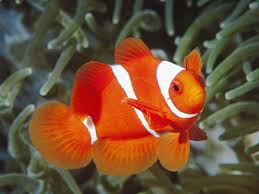
\includegraphics[width=0.95\textwidth]{nemo.jpeg} %% PARA COLOCAR O ARQUIVO DA IMAGEM NO SHARELATEX, CLIQUE NO ÍCONE QUE PARECE UMA FLECHINHA PARA CIMA (ATUALIZAR), CLIQUE EM UPLOAD E PROCURE A IMAGEM EM SEU COMPUTADOR.
\end{figure}



\section{Contexto e Problema}

Nesta sessão o aluno especificará qual o contexto onde o trabalho se encontra. Por exemplo, se for um trabalho na área de sistemas distribuídos, um possível contexto específico é a sub-área de middlewares, logo deverá falar um pouco deste conceito. 
Deverá ser dissertado aqui também qual o problema resolvido neste trabalho, porém apenas apresentando-o.


\section{Objetivos}

O objetivo da pesquisa deve ser diretamente verificável ao final do trabalho. Um bom objetivo de pesquisa
possivelmente irá demonstrar que alguma hipótese sendo testada é ou não verdadeira.
Portanto, o objetivo geral e os objetivos específicos do trabalho devem ser expressos na forma de uma
condição não trivial cujo sucesso possa vir a ser verificado ao final do trabalho. Um objetivo bem expresso em
geral terá verbos como “demonstrar”, “provar”, “melhorar” (de acordo com alguma métrica definida) etc.
Deve-se tomar cuidado com certos verbos que determinam objetivos cuja verificação é trivial e, portanto,
inadequada. Entre eles pode-se citar “propor”, “estudar”, “apresentar” etc. Se o objetivo do trabalho épropor
algo, basta que a coisa seja proposta para que o objetivo seja atingido e, portanto, essa forma é trivial e
inadequada, pois a definição do objetivo não menciona a qualidade daquilo que será proposto.
Se o objetivo do trabalho é estudar algo, então ele terá sido alcançado se aquilo foi estudado, não importando
se alguma nova informação foi aprendida ou não, sendo, portanto, inadequado como objetivo de pesquisa.
Estudar, normalmente, é o objetivo do aluno e não do trabalho.
Se o objetivo do trabalho consiste em apresentar algo, novamente ele é trivial e inadequado. Uma simples
apresentação não produz necessariamente conhecimento novo. Por exemplo, “o objetivo deste trabalho é
apresentar os operadores da lógica booleana”; tal objetivo pode ser alcançado com um pequeno texto
explicando os operadores conhecidos, mas, como não traz informação nova, não é um objetivo de pesquisa.
A proposta, o estudo e a apresentação podem ser justificáveis como objetivo de pesquisa desde que o objeto
da proposta, estudo ou da apresentação seja algo original.
Segundo Chinneck (1988), um TCC deve apresentar uma contribuição original ao conhecimento.
Dessa forma, ao final do trabalho, o estudante deverá ser capaz de mostrar que identificou um problema que
valia a pena ser resolvido, mas que ainda não havia sido. Além disso, o estudante deverá mostrar que ele
resolveu o problema que propôs e apresentar a solução.
Em função disso, Chinneck conclui que um avaliador, ao ler o texto de um TCC, vai procurar
responder às seguintes questões:
a) Qual é a questão de pesquisa que o aluno propôs?
b) É uma boa questão? (Já foi respondida alguma vez? Vale a pena respondê-la?)
c) O aluno conseguiu convencer que a questão foi respondida adequadamente?
d) O aluno fez uma contribuição adequada ao conhecimento?
A falha em encontrar respostas para alguma dessas questões poderá colocar o aluno em apuros, sendo que a
banca avaliadora provavelmente exigirá revisões extensas no trabalho ou poderá até reprovar o candidato.

% ---
% Capitulo de revisão de literatura
% ---
\chapter{Referencial Teórico}

Aqui o aluno irá apresentar o “jargão” utilizado ao longo do texto. 
É o capítulo que tem mais referências bibliográficas. Aqui também é incluído o
histórico daquilo que ocorreu com o tema. Por exemplo, quando o tema é “internet”,
é esperado que tenha uma explicação de onde surgiu, porque, e quais os
melhoramentos que foram criados ao longo dos anos. Não é necessário entrar
em detalhes. A idéia geral já é o suficiente.

% --- Seção dentro do capítulo
\section{Assunto Um}
% ---

Falar do assunto Um

% --- Seção dentro do capítulo
\section{Assunto Dois}
% ---

Falar do assunto Dois

% --- Seção dentro do capítulo
\section{Assunto N}
% ---

Falar do assunto Três

\chapter{Trabalhos Relacionados}

Lista trabalhos anteriores cujos temas sejam relacionados ao seu (forneça detalhes desses trabalhos apenas se tais detalhes ajudam a mostrar onde o seu trabalho é melhor do que eles; tenha certeza de mencionar todos os trabalhos relacionados, principalmente aqueles do pessoal do comitê de programa). Desvantagens ou pontos fracos de trabalhos anteriores que são aprimorados no trabalho sendo proposto. Condições e limitações do seu trabalho.


\chapter{Capítulo de Desenvolvimento}

O capítulo de desenvolvimento marca o início da contribuição pessoal do autor do trabalho. Portanto, não se
deve fazer do capítulo de desenvolvimento uma nova revisão bibliográfica. De preferência, todos os conceitos
que serão necessários nesse capítulo já devem ter sido citados no capítulo de revisão bibliográfica. Se alguma
comparação for feita com trabalhos correlatos nesse capítulo, então apenas a comparação objetiva deve ser feita
aqui, sendo que a apresentação pura e simples dos trabalhos correlatos já terá ocorrido no capítulo anterior.
O capítulo de desenvolvimento deve apresentar a construção da teoria, modelo ou proposta, seja de que
natureza for. Conceitos criados pelo autor do Trabalho de Conclusão de Curso devem ser descritos aqui e não na revisão
bibliográfica. Na sequência, o autor deve trabalhar as evidências de que sua hipótese é verdadeira. Serão então
apresentados dados, gráficos, testes, provas formais, estudos de casos, transcrição de entrevistas ou quaisquer
outros meios julgados adequados para provar o seu ponto, ou seja, para mostrar que a hipótese é verdadeira.
Deve-se evitar sempre transformar o capítulo de desenvolvimento em uma apresentação de um sistema
computacional. Se um sistema foi desenvolvido, foi para servir a algum propósito de descobrir novo
conhecimento. A monografia deve ser sobre o conhecimento gerado, não sobre o sistema em si. Apresentações
detalhadas sobre telas de software, incluindo telas de login, menu principal etc., são enfadonhas e
desnecessárias em um trabalho científico. O seguinte texto, do Prof. J ohn W.Chinneck (1988), resume tudo:
“The purpose of your thesis is to clearly document an original contribution to knowledge. You may develop computer
programs, prototypes, or other tools as a means of proving your points, but remember, the thesis is not about the tool, it is
about the contribution to knowledge. Tools such as computer programs are fine and useful products, but you can’t get an
advanced degree just for the tool. You must use the tool to demonstrate that you have made an original contribution to
knowledge; e.g., through its use, or ideas it embodies.”

\section{Avaliação/Estudos de Caso}

Nesta parte do trabalho o aluno deverá apresentar indicativos que sua proposta e ou suas hipóteses foram comprovadas através de uma análise prática. Esta atividade poderá ser feita seguindo métodos de experimentos controlados ou mais simplesmente estudos de caso.


% ---
% Conclusão
% ---
\chapter{Conclusão}

O capítulo das conclusões é, em geral, a pedra no sapato do estudante. Aparentemente tudo já foi dito sobre o
trabalho no capítulo de desenvolvimento; então o que escrever nesse capítulo final?
A primeira dica é observar os objetivos geral e específicos do trabalho no capítulo de introdução e colocar no
capítulo das conclusões um comentário sobre como o desenvolvimento apresentado ajudou a chegar a cada um
desses objetivos, ou seja, como o trabalho de pesquisa permite concluir que cada um dos objetivos foi atingido.
Outro ponto importante é apresentar não apenas os pontos positivos do trabalho, mas também os negativos.
Não se espera de nenhum trabalho científico que ele resolva todos os problemas do mundo. Pelo contrário,
espera-se que o pesquisador seja suficientemente honesto para descrever de forma clara as fraquezas e
limitações de seu próprio trabalho.
A seguinte máxima segue implacavelmente das leis da lógica: “Se você não for o maior crítico de seu próprio
trabalho, outra pessoa será”.
Outro tópico a ser abordado no capítulo de conclusões são as lições aprendidas. O aluno passou dois anos ou
mais estudando um tema e realizando experimentos com ele. Além dos objetivos do trabalho, claramente
colocados e atingidos, ele deve ter aprendido muita coisa no processo. Talvez essa informação possa ser útil a
outras pessoas. Então se deve descrever no capítulo de conclusões quais foram essas lições aprendidas ao longo
do trabalho.
Pode-se descrever também outras situações nas quais se imagina que essas lições possam ser aplicadas. Por
exemplo, ao comparar o resultado de questionários aplicados em uma empresa com a situação real observada in
locu, um aluno percebeu que, por conta do medo de retaliações por parte da chefia, a maioria dos funcionários
procurava apresentar nos questionários uma situação mais bonita do que realmente era. Dessa forma, o aluno
aprendeu que questionários não são fontes confiáveis de informação se não houver uma validação das
respostas no ambiente de estudo. Essa lição aprendida teria de ser colocada no capítulo de conclusões.
(1988), o capítulo final de um TCC deve ter pelo menos três partes: a conclusão, as contribuições e os
trabalhos futuros.
Na conclusão o aluno fará de forma concisa uma referência ao problema examinado e resolvido. A conclusão
propriamente dita teria o seguinte formato: “o problema descrito na seção x foi resolvido como demonstrado
nas sessões y a z, em que foi desenvolvido um algoritmo/método/abordagem etc. para tratar as situações
mencionadas” (Chinneck, 1988).
Ainda segundo Chinneck, o resumo das contribuições, que viria em seguida, deve ser organizado em ordem
decrescente de sua importância, por exemplo:
a) Desenvolveu-se um algoritmo muito mais rápido para problemas de Zylon de grande porte.
b) Demonstrou-se pela primeira vez o uso do mecanismo de Grooty para os cálculos de Zylon.
c) Etc.
As contribuições mais importantes do trabalho serão aquelas que geraram conhecimento novo. Ferramentas,
protótipos e outros artefatos tecnológicos usualmente são contribuições secundárias.
Artigos publicados e relatórios de pesquisa não são contribuições, nesse sentido da palavra, mas relatos da
pesquisa. Portanto, tais referências não deveriam ser mencionadas aqui.
Finalmente, os trabalhos futuros são a contribuição que o aluno deixa para que outros possam continuar sua
pesquisa. Trabalhos futuros também devem tratar de futuras contribuições ao conhecimento com mais ênfase
do que futuras contribuições às ferramentas, protótipos etc., que eventualmente possam ser desenvolvidas.


\chapter{Publicações}
Caso o aluno possua publicações de artigos científicos, estes deverão ser listados neste capítulo.

% ----------------------------------------------------------
% ELEMENTOS PÓS-TEXTUAIS
% ----------------------------------------------------------
\postextual


% ----------------------------------------------------------
% Referências bibliográficas
% ----------------------------------------------------------
\bibliography{references} %% REFERENCIA AO ARQUIVO abntex2-modelo-references.bib

% ----------------------------------------------------------
% Glossário
% ----------------------------------------------------------
%
% Consulte o manual da classe abntex2 para orientações sobre o glossário.
%
%\glossary

% ----------------------------------------------------------
% Apêndices
% ----------------------------------------------------------

% ---
% Inicia os apêndices
% ---
\begin{apendicesenv}

% Imprime uma página indicando o início dos apêndices
\partapendices

% ----------------------------------------------------------
\chapter{Apêndice}
% ----------------------------------------------------------


\end{apendicesenv}
% ---



\end{document}
